\documentclass[12pt]{article}

\usepackage[paper=a4paper,left=25mm,right=25mm,top=25mm,bottom=25mm]{geometry}
\usepackage{url}
\usepackage{notoccite}
\usepackage{graphicx}
\usepackage{multirow}
\usepackage{verbatim}
\graphicspath{ {images/} }

%opening
\title{Cloud Computing Project - Analyzing the connection between flights and cases of Covid-19 in Europe: Specifications}
\author{Aeilko Lübsen, Gonçalo Antunes, Cláudio Lamelas, Rafael Oliveira}

\begin{document}
	\maketitle
	
	Our goal for this project is to implement a system that provides an API, which analyzes the connection between cases of Covid-19 and and international flight in Europe. To do this, we use datasets on flights, Covid-19-cases and airports \cite{airtraffic2021, covid2022, nuts2016, airports2022}. Our backend is supposed to be used by a frontend, which shows a heatmap of Covid-19-cases and flights that could be controlled by a slider changing the date of what is shown. The use cases are displayed in Figure~\ref{fig:use_cases}. Because we assume that this application would be quite processing-intensive we also include a use case for administrators to monitor and analyze network data sizes and request runtimes.
	
	\begin{figure}[h!]
		\centering
		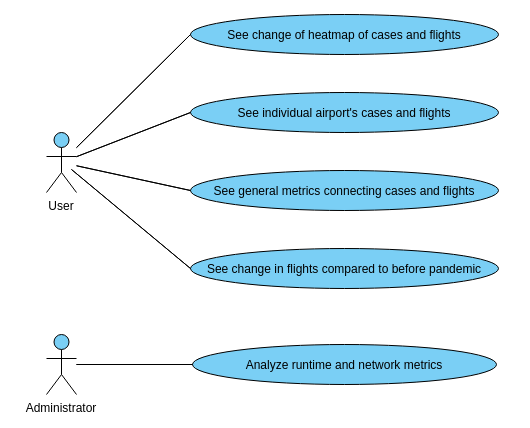
\includegraphics[scale=0.6]{use_cases.png}
		\caption{Use case diagram for the system.}
		\label{fig:use_cases}
	\end{figure}

	Figure~\ref{fig:architecture} shows our preliminary microservice architecture for the system. It only exposes a single API to the outside user, which is optimized to be used by a specific frontend. Behind this API are five different microservices. Two of the microservices directly concern the data from the datasets. The data delivery service reads flight and case data from the database and forwards it to the API, while data analysis microservice performs statistical operations to gain deeper insights into the gathered data. Both of these services also write their runtime and network size metrics into the database, so the administrator analysis microservice can analyze and pass it to the outbound API. To secure this data, there is an authentication microservice. Also, as according to the 12-factor pattern there is a separate logging microservice. As a database management system, we intend to use PostGIS to best support the required geographical operations. This database will be filled automatically by an ingestion pipeline that downloads the datasets from the web, parses the files and inserts the data.
	
	\begin{figure}[h!]
		\centering
		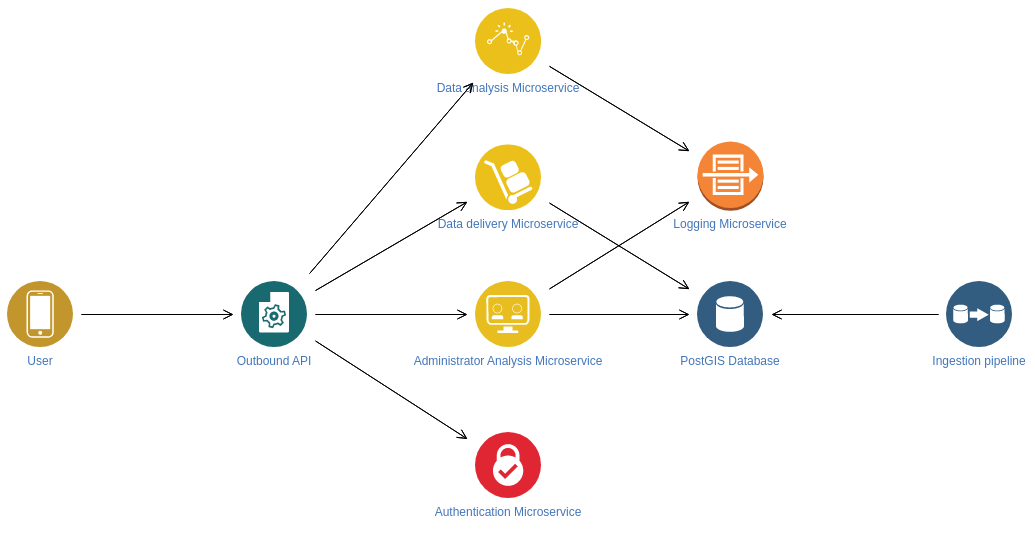
\includegraphics[scale=0.38]{architecture.png}
		\caption{Preliminary architecture for the system.}
		\label{fig:architecture}
	\end{figure}

	\bibliographystyle{unsrt}

	\bibliography{references}
	
\end{document}